\section{Dispositif: Effet Tcherenkov par des électrons}
\label{sect:Tcherenkov_electron}

L'effet Tcherenkov survient lorsqu'une particule chargée se déplace plus vite que la vitesse de la lumière dans un milieu diélectrique. Ce phénomène résulte de la superposition cohérente d'onde électromagnétique suite à la polarisation du milieu par le passage de la particule chargée. Si la vitesse de la particule est supérieure au ratio $c/n$ (où $n$ est l'indice de réfraction et $c$ la vitesse de la lumière dans le vide), il y a formation d'un cône de lumière avec un angle de demi-ouverture $\Theta_c$ qui suit la relation:

\begin{equation}
    cos\Theta_c = \frac{1}{n\beta}
\end{equation}\\
où $\beta = v/c$, $v$ étant la vitesse de la particule dans le milieu. Le nombre de photons Tcherenkov émis par unité de longueur et de longeur d'onde est donné par la formule de Frank-Tamm:
\begin{equation}
     \frac{d^2N}{dx \, d\lambda} = \frac{2\pi \, \alpha}{\lambda^2} \; (1- \frac{1}{n^2 \, \beta^2} )
\end{equation}\\
avec $\alpha$ étant la constante de structure-fine. Comme le nombre de photons produits est inversement proportionnel à la longueur d'onde, la contribution des petites longueurs d'onde est plus importante.

Cette manipulation a pour but la caractérisation d'un module optique (OM) développé pour l'expérience AMANDA. AMANDA (Antarctic Muon and Neutrino Detector Array) était  un télescope à neutrino localisé au Pôle Sud. Lors de sa phase finale, le détecteur était composé de 677 modules optiques (OMs) disposés sur 19 câbles. Il avait pour but principal la détection des neutrinos à haute énergie. Compte tenu de leur faible section efficace d'interaction, la détection des neutrinos nécessite un détecteur de grand volume. Cela est réalisé par les détecteurs Tcherenkov en déployant des photo-multiplicateurs (PMs) dans un volume de matériau diélectrique. Chaque PM est contenu dans une bulle de verre sous vide, l'ensemble étant appelé module optique (OM). Après 9 ans d'activité, AMANDA a été officiellement incorporé au détecteur IceCube en 2005. IceCube (figure~\ref{fig:IceCube1}) est un détecteur Tcherenkov d'un kilomètre cube enterré dans la glace du Pôle Sud. IceCube est composé de 5160 modules optiques digitaux (DOMs ou Digital Optical Modules) placés sur 86 câbles. Dans le cas d'AMANDA et IceCube, le matériau diélectrique est la glace, alors que l’eau est aussi fréquement utilisée, par exemple à l'observatoire Pierre Auger, qui mesure des rayons cosmiques aux plus hautes énergies. Dans notre dispositif, nous utilisons du quartz.

Pour constituer un vaste réseaux d'OMs, il nous faut connaître la réponse de chacun de ceux-ci. Afin d'étudier les propriétés de cet OM, vous devrez mettre au point le dispositif nécessaire à la prise de mesure. Après avoir pris connaissance avec le dispositif, vous serez ainsi amené à développer vous même la logique d'acquisition des données. Vous analyserez ensuite les données recueillies grâce aux outils statistiques et informatiques que vous aurez vu en cours.

\begin{figure}
    \center{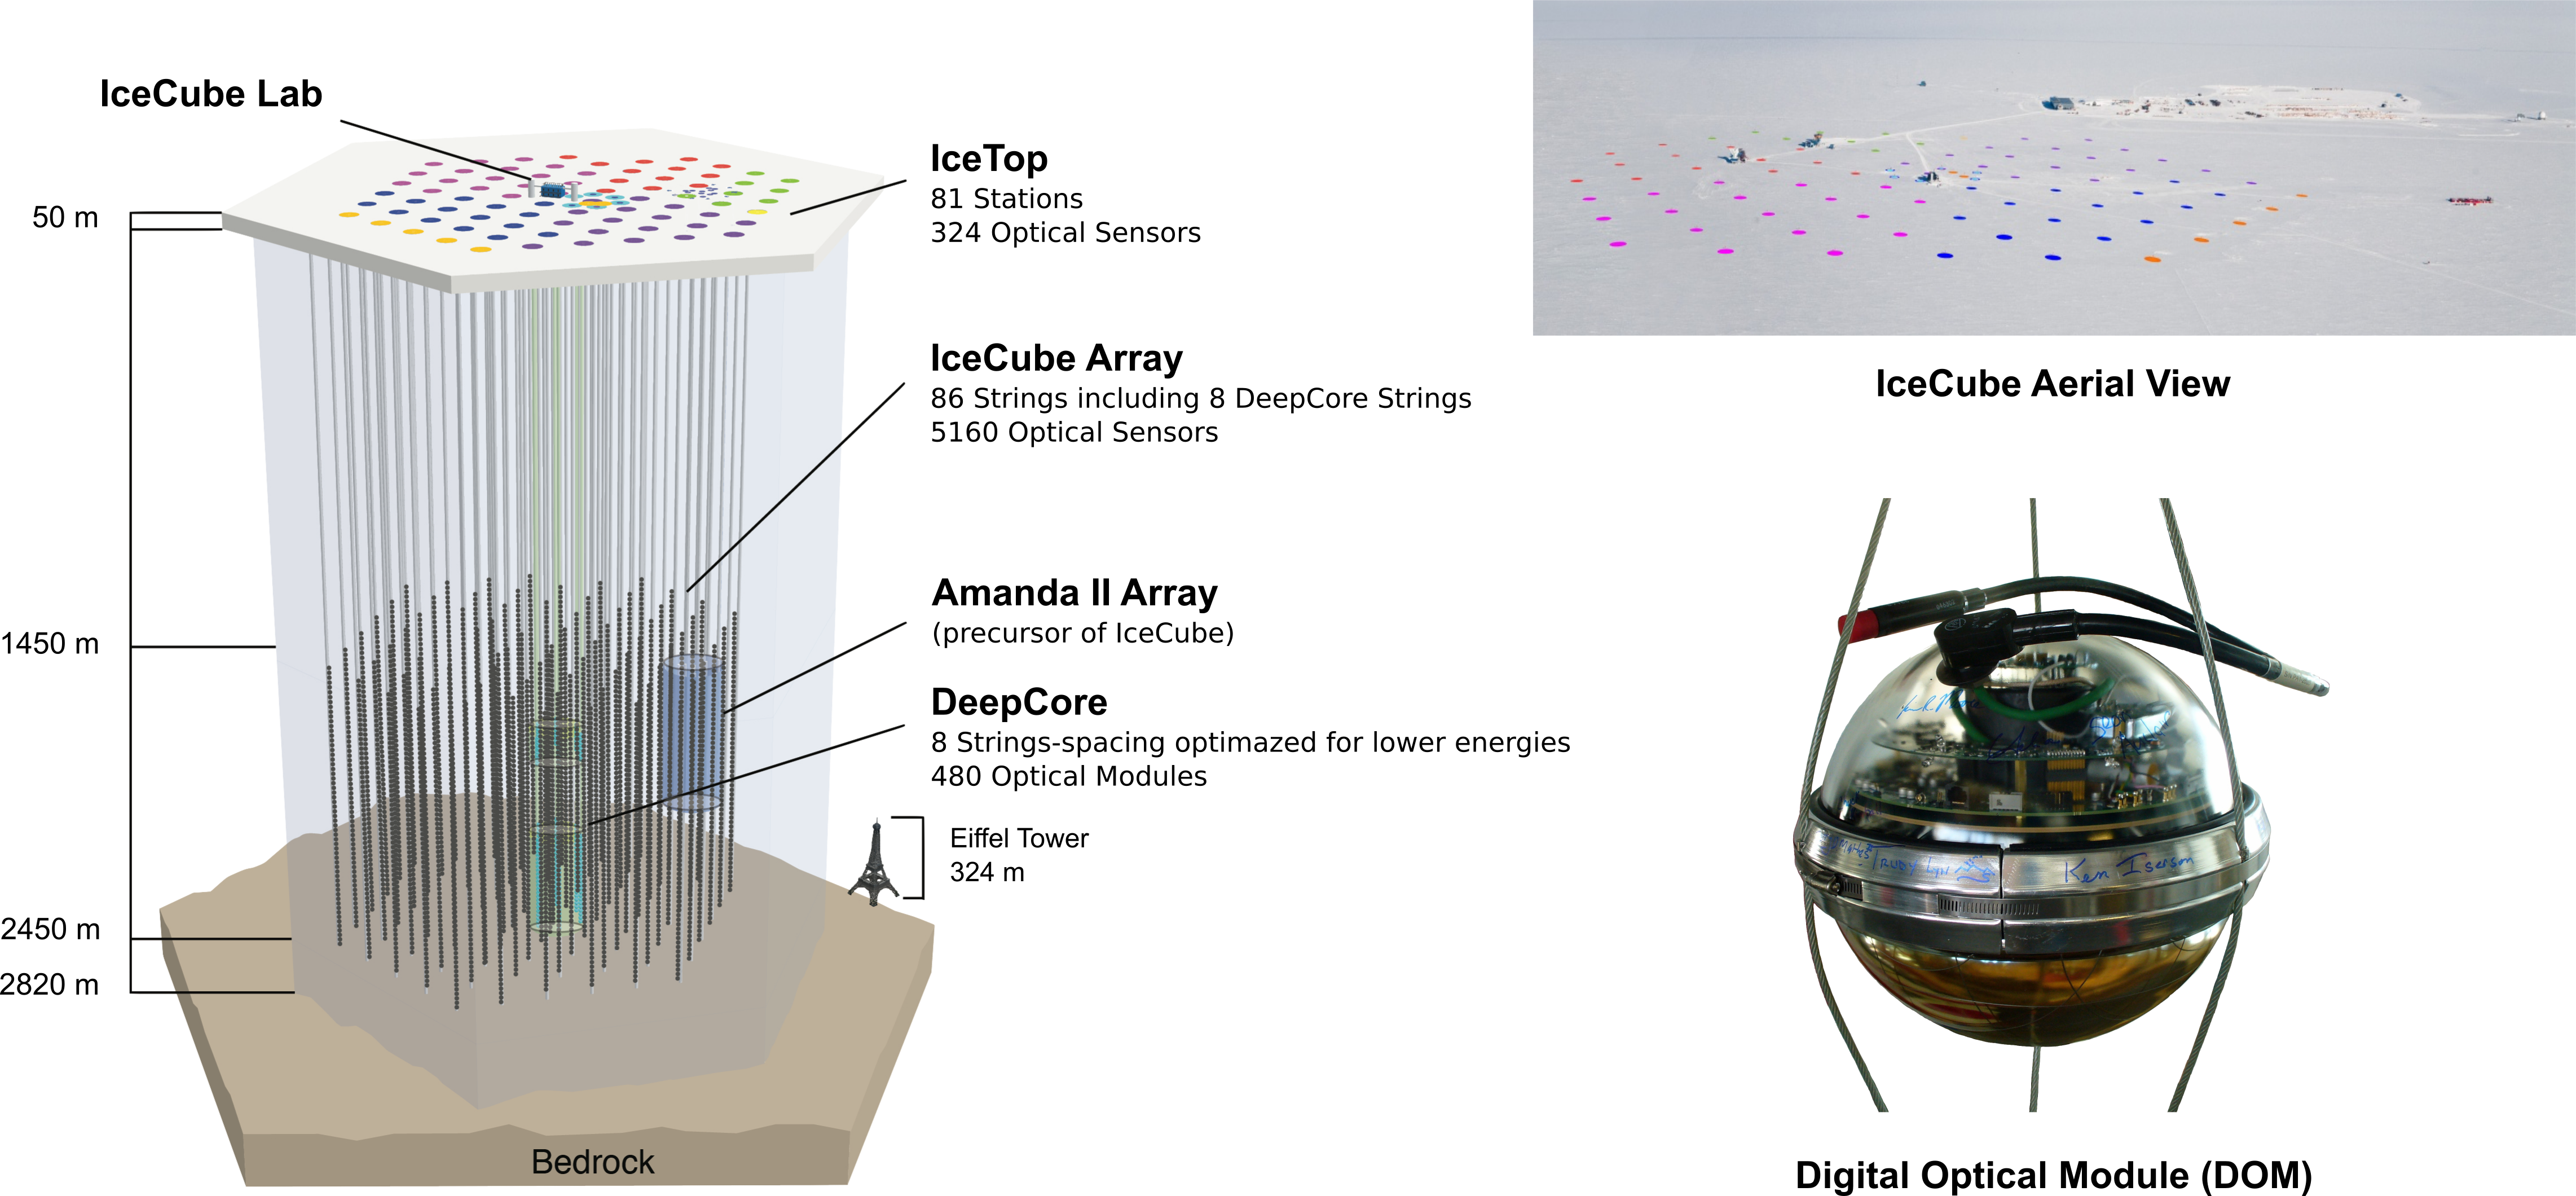
\includegraphics[width=0.8\textwidth]
    {figures/IceCube_Detector.png}}
    \caption{\label{fig:IceCube1} Configuration du télescope à neutrinos IceCube.}
\end{figure}

\subsection{Agenda du laboratoire}
\begin{tabular}{p{0.2\linewidth} p{0.8\linewidth}}
Lundi & - Prise de connaissance avec le matériel\newline
		- Vérification du signal analogique des PMs avec l'oscilloscope\newline
		- Implémentation de la table de vérité pour la logique d'acquisition ou trigger\newline
		- Mesure de l'efficacité\\

Mardi & - Calibration de l'ADC\newline
		- Préparation de l'acquisition de données\newline
		- Début de l'acquisition de données avec LabView\\

Mercredi & - Construction de la logique d'acquisition du bruit de fond\newline
		- Écriture de la table de vérité pour définir un événement du bruit\newline
		- Début de l'acquisition de données pour le bruit de fond\\

Jeudi et Vendredi & - Développement d'un programme de génération MC d'une distribution normale\newline
		- Développement des programmes d'analyse\newline
		- Dernier jour pour présenter les résultats des exercices\newline
		- Préparation de la présentation\newline
\end{tabular} 

\subsection{Dispositif expérimental}
Cette manipulation utilise une source de radiation $\beta^+$ composée de Strontium $^{90}$Sr. Les électrons émis par la source traverse ensuite une plaque de quartz d'indice de réfraction  $n = 1.478$. Lors de leur passage, les électrons vont produire un rayonnement Tcherenkov qui pourra être détecté par l'OM. Dans ce dispositif, l'OM se trouve à une position fixe située à un angle de 45$^{\circ}$ par rapport à la direction d'émission des électrons (voir figure \ref{fig:dispo1}). La source radioactive est combinée à un spectromètre qui va nous permettre de sélectionner l'énergie cinétique des électrons afin de récolter un maximum de rayonnement Tcherenkov dans l'OM. Pour déterminer l'intensité du courant à fournir au spectromètre pour obtenir des électrons de cette énergie, vous devrez d'abord résoudre l'exercice 1.

Une fois cette valeur trouvée, vous pouvez allumer le spectromètre. Celui-ci est calibré sur la partie descendante de la courbe d'hystérèse, il vous faudra donc respecter les conditions d'utilisation décrites ci-dessous.

\textbf{Mode d'emploi du spectromètre :}
\begin{quote}
    \begin{itemize}
        \item Démarrez à $I$ = 0 A
        \item Aller à saturation $I$ $\sim$ 2,6 A
        \item Descendre à la valeur $I_t$ désirée
    \end{itemize}
\end{quote}
\textbf{Remarque :} Si on veut changer $I_t$ pour une valeur plus petite, on descend vers cette valeur. En revanche, si on veut augmenter cette valeur, on doit recommencer le cycle d'hystérèse. 

\begin{figure}
    \centering
    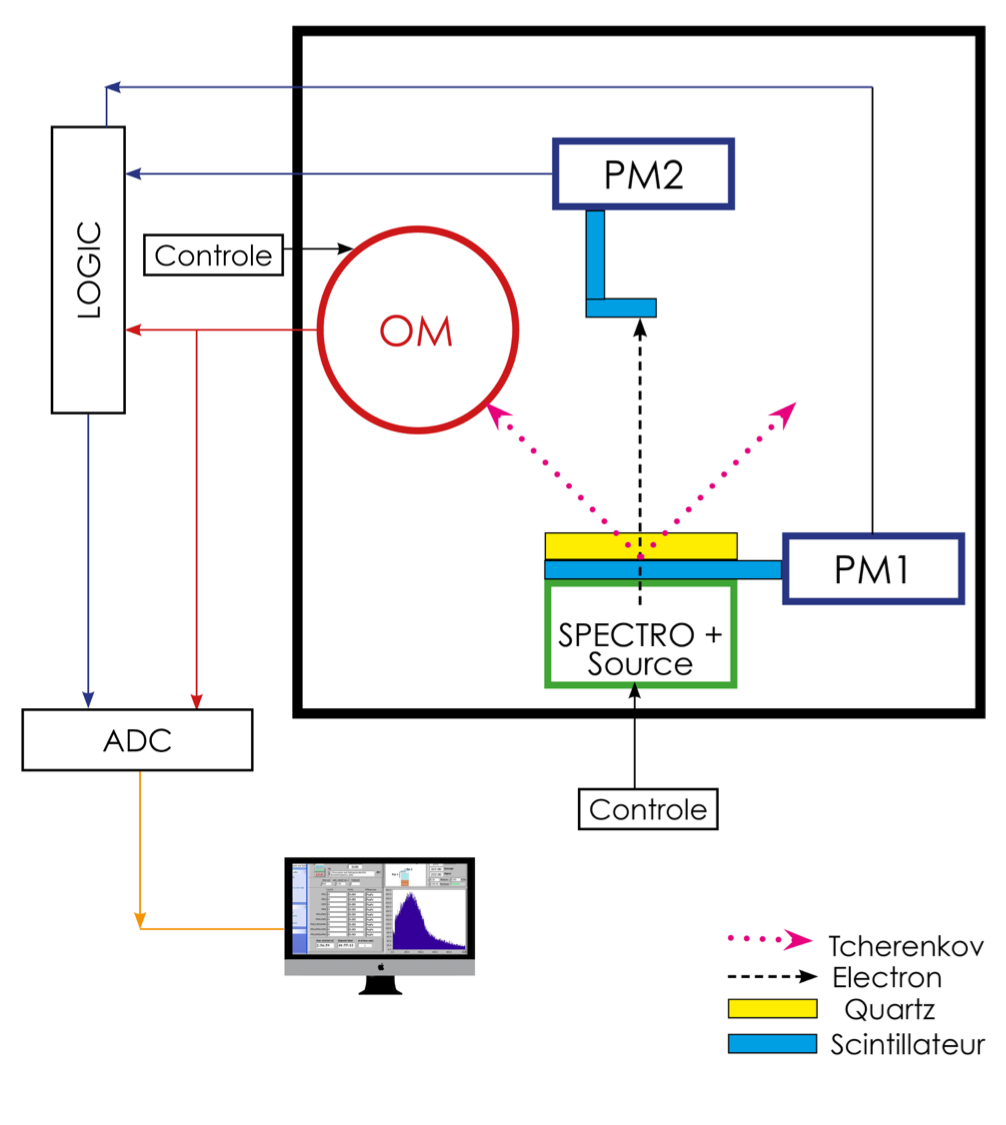
\includegraphics[width=0.5\textwidth]{figures/Dispositif_1.png}
    \caption{Dispositif expérimental de l'effet Tcherenkov produit par des électrons.}
    \label{fig:dispo1} 
\end{figure}

Dans ce dispositif, sont également présent 2 photo-multiplicateurs (PMs) chacun relié à un scintillateur. Le premier (PM1) est situé entre la source et la plaque de quartz et nous permet de vérifier qu'un électron a été émis par la source. Le second PM confirme que l'électron a bien traversé le quartz. Ces PMs ont donc pour but d'assurer que le signal détecté par l'OM est en coïncidence avec un électron qui a produit des photons Tcherenkov.


\subsection{Exercices Préparatoires}
\subsubsection{Exercice 1}
Sachant que l'OM est placé à un angle de $45^\circ$ par rapport à la direction d'émission des électrons ($m_\mathrm{e} = 0.511$\,MeV/$c^2$) de la source de strontium, à quel courant faut-il régler le spectromètre pour récolter un maximum de rayonnement Tcherenkov dans l'OM, sachant que l'indice de réfraction du quartz est de $1.478$?
Le graphique suivant vous donne la relation entre l'énergie cinétique des électrons et l'intensité du courant.
\begin{center}
	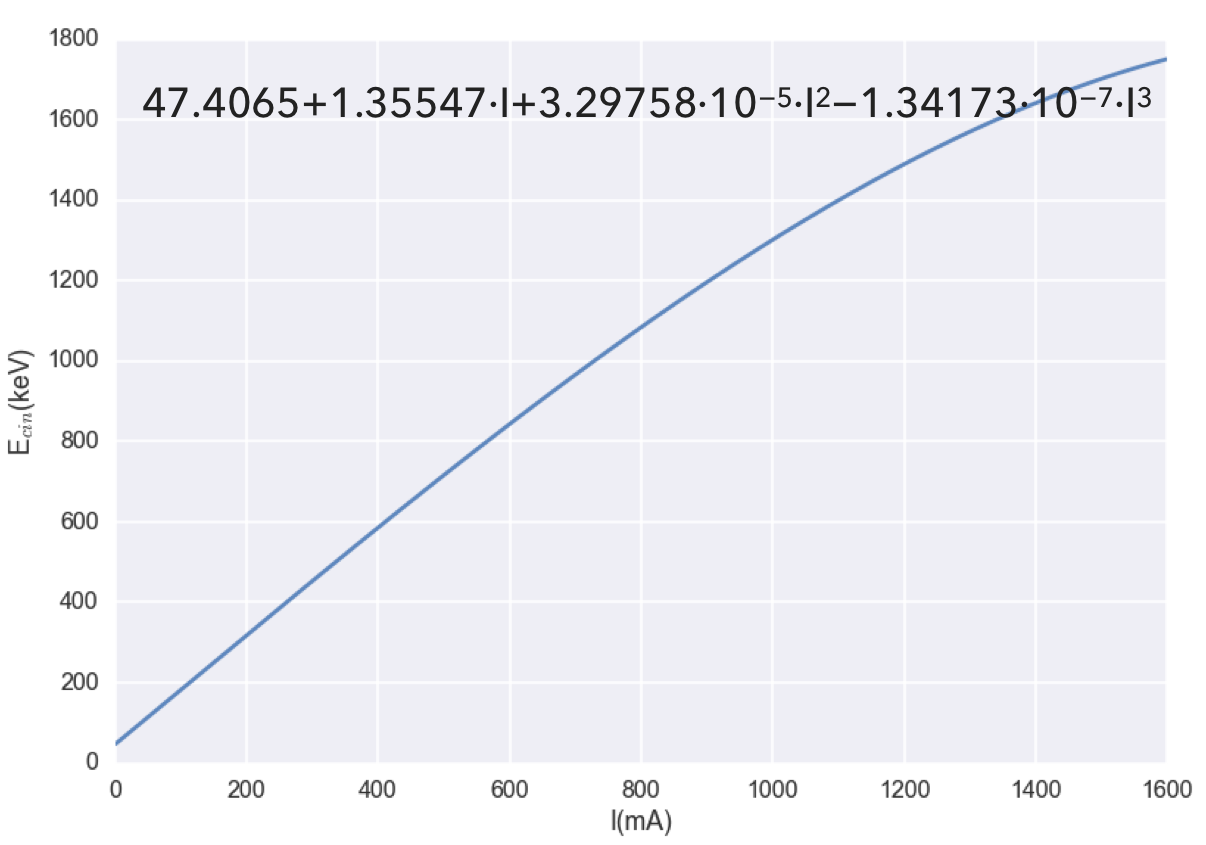
\includegraphics[width=0.5\textwidth]{figures/Relation_Ecin_I.png}
\end{center}

\ifthenelse{\boolean{showAdditional}}{
\begin{additional}
\begin{align*}
\beta &= \frac{1}{n\cos\Theta_\mathrm{c}} = 0.9568\\
 &= \frac{pc}{E}\\
 &= \frac{\sqrt{E^2-m_\mathrm{e}^2c^4}}{E}\\
 &\\
E &= \sqrt{\frac{m_\mathrm{e}^2c^4}{1 - \beta^2}} = 1.7575\,\mathrm{MeV}\\
E_\mathrm{cin}&=E- m_\mathrm{e}\\
 &= 1.247\,\mathrm{MeV} \\
&\Rightarrow \boxed{I \approx 950\,\mathrm{mA}} \\
\end{align*}
\end{additional}
}

\subsubsection{Exercice 2}
Calculer l'ordre de grandeur du nombre de photons émis entre $350$ et $500$\,nm par un électron de $1247$\,keV d'énergie cinétique traversant une fenêtre de quartz de 1\,mm d'épaisseur. Pour ce domaine de longueurs d’onde, l'indice de réfraction du quartz varie de moins de 1\% et peut être considéré constant ($1.478$). Négliger la perte d'énergie de l'électron dans le quartz.\\ $\alpha = 1/137$

\ifthenelse{\boolean{showAdditional}}{
\begin{additional}
Formule de \emph{Frank-Tamm}:
\begin{align*}
\frac{\mathrm{d}N}{\mathrm{d}x} &= \int_{\lambda_0}^{\lambda_1} \frac{2\pi\alpha z^2}{\lambda^2} \sin^2\Theta_\mathrm{c} \mathrm{d}\lambda\\
&=\frac{\pi}{137}\int_{350\,\mathrm{nm}}^{500\,\mathrm{nm}}\frac{\mathrm{d}\lambda}{\lambda^2}\\
N&=\frac{\pi}{137}\cdot\left(\frac{1}{350\,\mathrm{nm}}-\frac{1}{500\,\mathrm{nm}}\right)\cdot1\,\mathrm{mm}\\
&=\boxed{19.65}
\end{align*}
\end{additional}
}

\subsubsection{Exercice 3}
En supposant que le diamètre du collimateur placé devant la photocathode de l'OM est de 6 cm et qu'il se trouve à 17\,cm de la fenêtre de quartz, combien de photoelectrons l'OM peut-il enregistrer par électron de la source, en supposant une transmittance $T$ de 90\% et sachant que l'efficacité quantique est de $\epsilon_\mathrm{q}=15\%$?

\ifthenelse{\boolean{showAdditional}}{
\begin{additional}
Avec $N_\mathrm{\gamma}^{\mathrm{quartz}}$ trouvé avant, on obtient:
\begin{align*}
N_{\mathrm{pe}} &= \epsilon_\mathrm{q} \cdot T \cdot N_\mathrm{\gamma}^{\mathrm{OM}}\\
 &= \epsilon_\mathrm{q} \cdot T \cdot \frac{6\,\mathrm{cm}}{2\pi \cdot 17\,\mathrm{cm} \cdot\sin\Theta_\mathrm{c}} \cdot N_\mathrm{\gamma}^{\mathrm{quartz}}\\
&= \boxed{3.58}
\end{align*}
\end{additional}
}

\subsection{Prise de mesure}
Pour cette manipulation, il vous est demandé de préparer le dispositif expérimental nécessaire à la prise de mesure. Cela implique, dans un premier temps, de :
\begin{center}
\fbox{
\begin{minipage}{0.75\textwidth}
\textbf{Se familiariser avec le dispositif :} 
\begin{quote}
\begin{itemize}
\item vérifier le signal des différents PMs et de l'OM
\item étudier l'efficacité des PMs
\item calibrer l'ADC
\item développer la logique d'acquisition de données
\item mesurer le bruit de fond
\end{itemize}
\end{quote}
\end{minipage}
}
\end{center}

\subsubsection{Vérification du dispositif}
Dans un premier temps, allumez votre dispositif et allumez la haute tension aux bornes des PM. Veillez à ne pas changer la tension indiquée afin de ne pas endommager les PMs.

Après avoir calculé l'intensité du courant à fournir au spectromètre, allumez également celui-ci en suivant les instructions fournies précédemment.

A l'aide de l'oscilloscope, vérifiez le signal provenant des différents photo-multiplicateurs (PMs) et de l'OM. Transformez ensuite votre signal analogue en signal digital à l'aide du discriminateur et observez celui-ci sur l'oscilloscope.

\subsubsection{Mesure de l'efficacité}
Il vous est ensuite demandé de mesurer l'efficacité d'un des PMs présents dans votre dispositif. Vous devrez faire cette mesure en faisant varier dans un premier temps le seuil du PM pour lequel vous mesurer l'efficacité. Une fois la valeur optimale du seuil trouvée, répétez le processus en faisant cette fois varier la tension appliquée sur le PM en question. Pour ces deux mesures, veillez également à mesurer le taux d'évènements détectés par le PM dont vous mesurez l'efficacité. Pour effectuer ces mesures, vous avez à votre disposition un scaler NIM. De quel PM allez-vous mesurer l'efficacité ?

\ifthenelse{\boolean{showAdditional}}{
\begin{additional}
\begin{itemize}
\item Mesure de l'efficacité de PM1
\item Logique : (PM1 \& PM2 \& OM) et (PM2 \& OM)
\item Mesure du rate de PM1
\end{itemize}
\end{additional}
}

\subsubsection{Calibration de l'ADC}
Nous allons à présent procéder à la calibration du convertisseur analogique-numérique (ADC ou Analogue-to-Digital Converter). En effet, l'ADC vous donne des valeurs en ADC channel, il vous faut donc connaître à quelle charge équivaut un ADC channel.

Pour cette calibration, il faut fournir une charge connue et constante à l'ADC. Pour cela, vous avez à votre disposition un générateur de courant continu. Comment allez-vous procéder ? 

\ifthenelse{\boolean{showAdditional}}{
\begin{additional}
\begin{itemize}
    \item Charge de l'ADC de l'ordre du pC $\to$ $Q\sim100$\,pC 
    \item Utilisation d'une résistance: $U = RI$ avec $R = 2.2$\,k$\mathrm{\Omega}$
    \item Sachant que $Q = I\mathrm{\Delta}t$, déterminer $\mathrm{\Delta}t$
    \item Le gate est ensuite créé à l'aide du dual-timer
\end{itemize}
\end{additional}
}

\subsubsection{Prise de données}
Afin de prendre les données nécessaires à la caractérisation de l'OM, nous devons réfléchir à la logique d'acquisition. Nous allons utiliser l'ADC que nous venons de calibrer et lui fournir le signal de l'OM ainsi qu'une porte logique (gate). Pour créer ce gate, nous avons besoin des modules logiques. Il nous faut réfléchir aux conditions dans lesquelles ont veut déclencher la prise de mesure. En d'autres termes, quand voulons nous considérer le signal de l'OM?

Une fois que vous avez déterminé cela, vous pouvez implémenter votre logique à l'aide des modules à votre disposition. Il vous faudra ensuite vérifier que le signal de l'OM et votre porte logique sont en coïncidence à l'aide de l'oscilloscope. Lorsque vous avez effectué cette vérification, reliez le gate et le signal de l'OM à l'ADC pour commencer acquisition.

Ayant plus d'évènements, la prise de mesure pour cette manipulation est très rapide. De ce fait, il vous sera demandé d'effectuer plusieurs mesures en faisant varier la tension.

\ifthenelse{\boolean{showAdditional}}{
\begin{additional}
\begin{itemize}
\item \textbf{Gate :} PM1 \& PM2 \& OM
\item Faire passer le gate dans le dual-timer pour avoir des fenêtres de tailles constantes
\item Vérifier que l'OM est en même temps que le gate
\item Donner les deux infos à l'ADC et prendre les mesures
\item Prendre des mesures en fonction de la tension pour voir la variation de la position du pic de 1 pe
\end{itemize}
\end{additional}
}

\subsubsection{Mesure du bruit de fond}
Intéressons nous au bruit de fond présent dans cette manipulation. Nous voulons connaître le taux de fausses coïncidences, càd les cas où l'OM nous envoie un signal qui n'est pas dû à un photon Tcherenkov alors que notre porte logique s'est déclenchée.

Dans un premier temps, il vous faut réfléchir à la manière dont vous pouvez implémenter la prise de mesure du bruit de fond. Une fois cette méthode mise en place, vous pouvez démarrer l'acquisition du bruit de fond. A l'aide de l'oscilloscope, pensez toutefois à vérifier que le signal de l'OM et votre gate arrivent en même temps à l'ADC.

\ifthenelse{\boolean{showAdditional}}{
\begin{additional}
\begin{itemize}
\item \textbf{Gate :} PM1 \& PM2 \& OM$_{\mathrm{couvert}}$
\item L'OM n'étant pas fixé au reste du dispositif, il est possible de le séparer physiquement à l'aide d'une couverture
\end{itemize}
\end{additional}
}

\subsection{Analyse de donn\'ees}
A présent, nous pouvons nous concentrer sur l'analyse des données dans le but de caractériser l'OM.

En vous basant sur les données, vous devrez calculer:
\begin{center}
\fbox{
\begin{minipage}{0.75\textwidth}
\begin{itemize}
\item le gain $G = \mu_{\text{best}}/e$ de l'OM,
\item la r\'esolution $\sigma_\mathrm{G} = \sigma_{\text{best}} / \mu_{\text{best}}$ de l'OM,
\item le nombre moyen de photo-\'electrons $\langle n_{\mathrm{pe}}\rangle$ produit par trigger dans l'OM.
\end{itemize}
\textbf{Remarque:} Mettez en graphique tout les ajustements ainsi que le gain et la résolution en fonction de la tension.
\end{minipage}
}
\end{center}

\ifthenelse{\boolean{showAdditional}}{
\begin{additional}
\textbf{Validation de la procedure d'adjustement:}\\
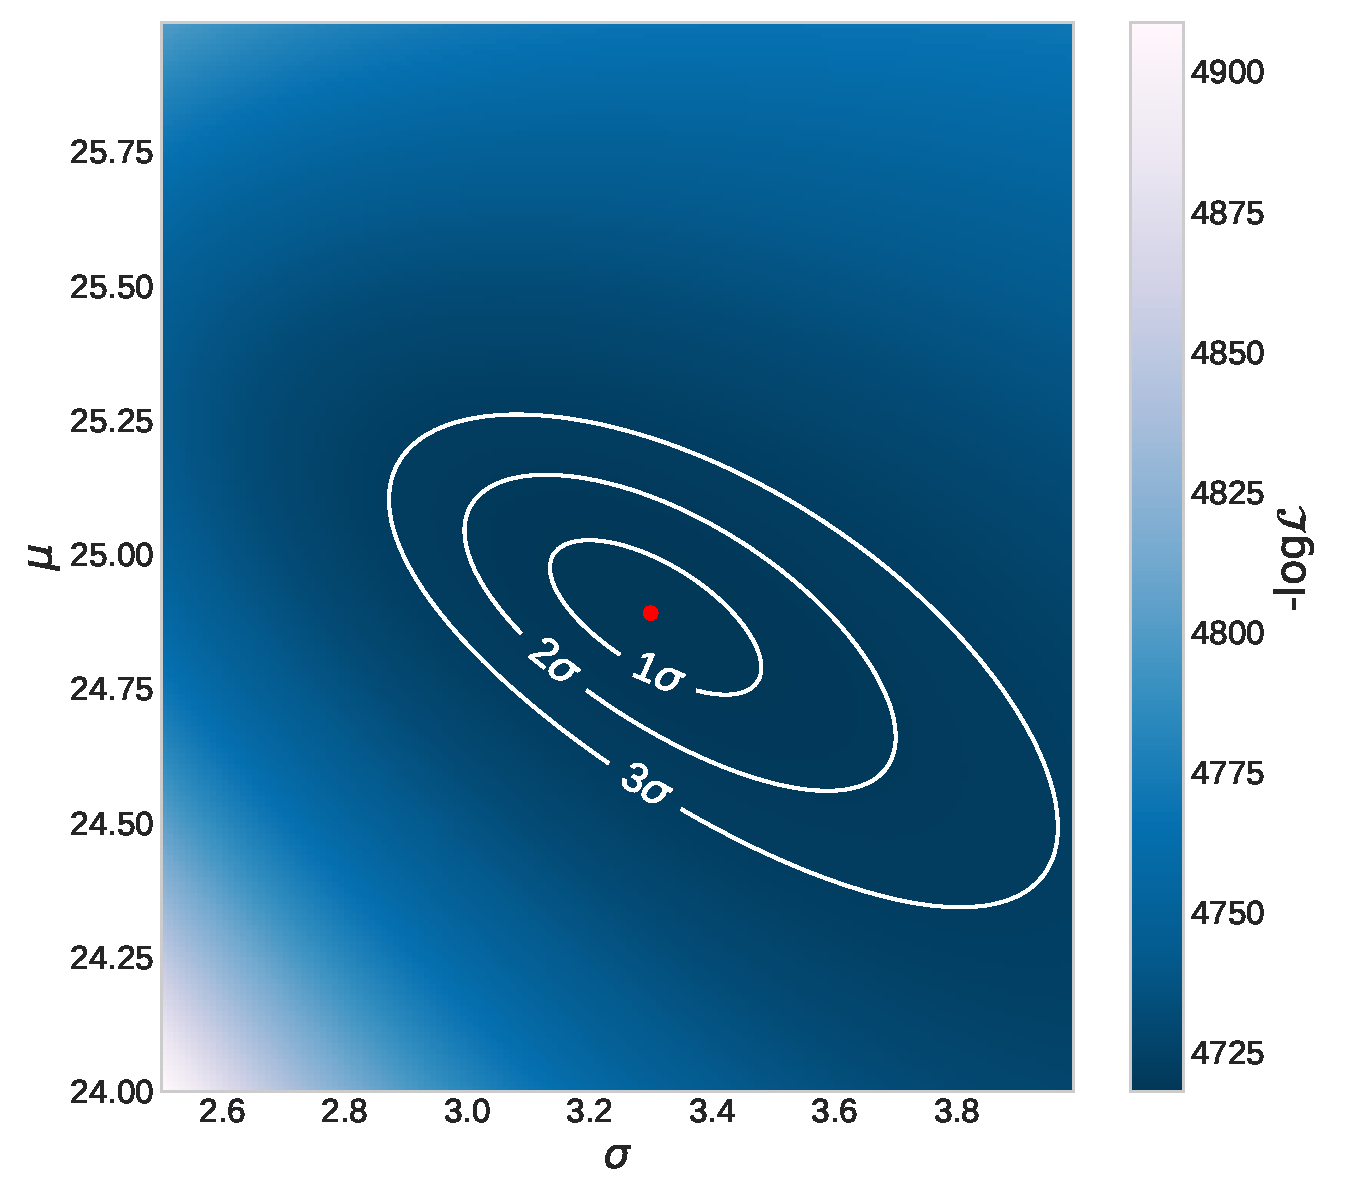
\includegraphics[width=0.45\textwidth]{exampleAnalysis/plots/Likelihood_MC.pdf}
\hfill 
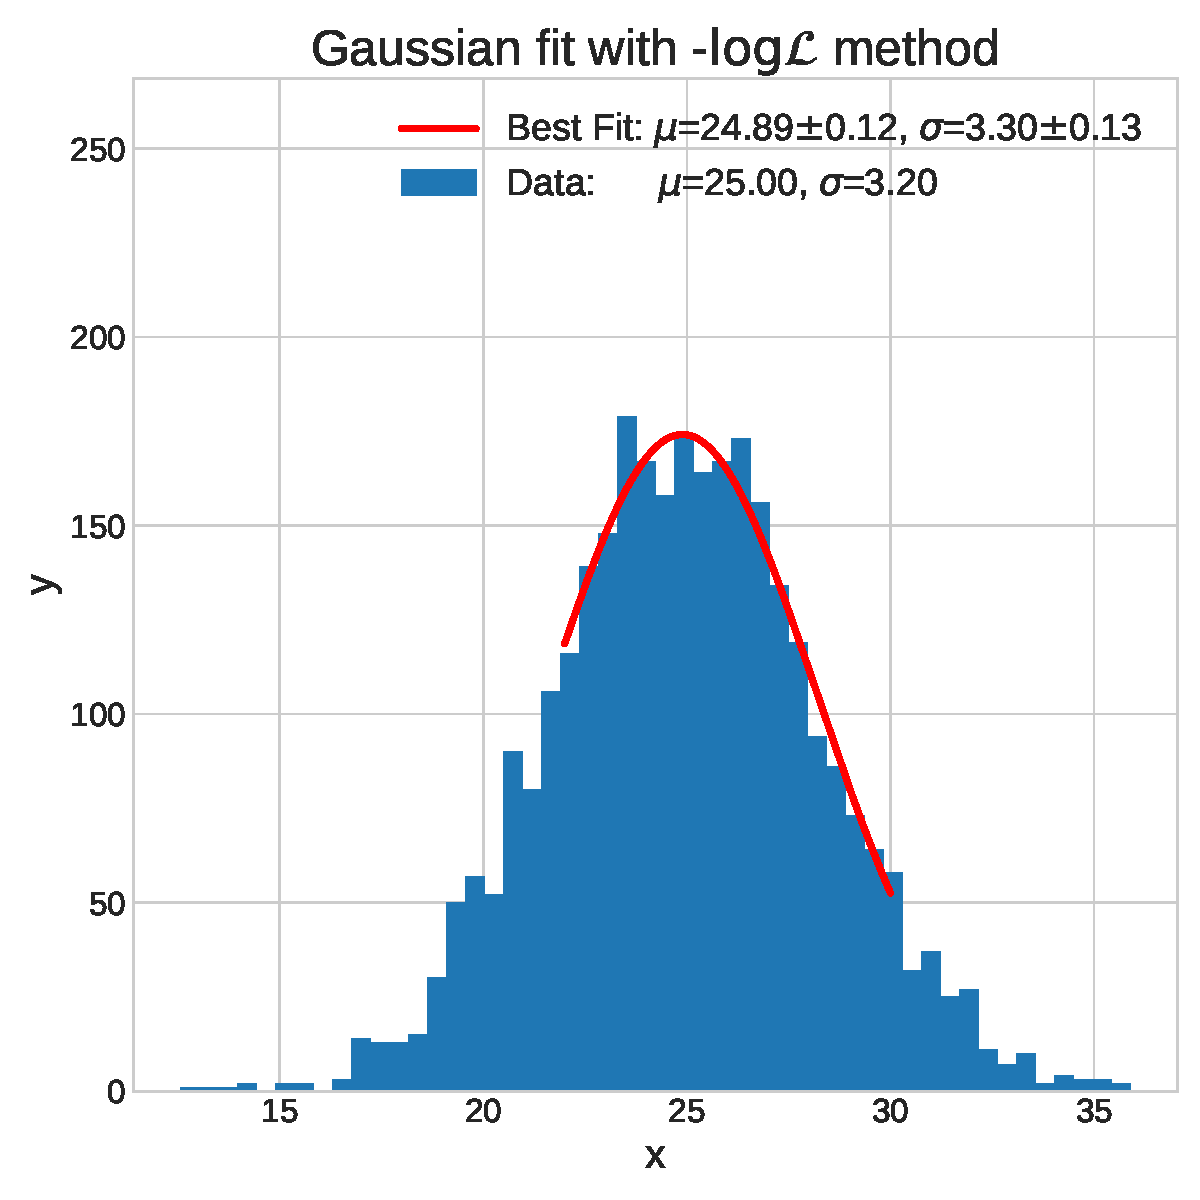
\includegraphics[width=0.45\textwidth]{exampleAnalysis/plots/LLH_Fit_MC.pdf}\\

\textbf{Ajustement des donn{\'e}es:}\\
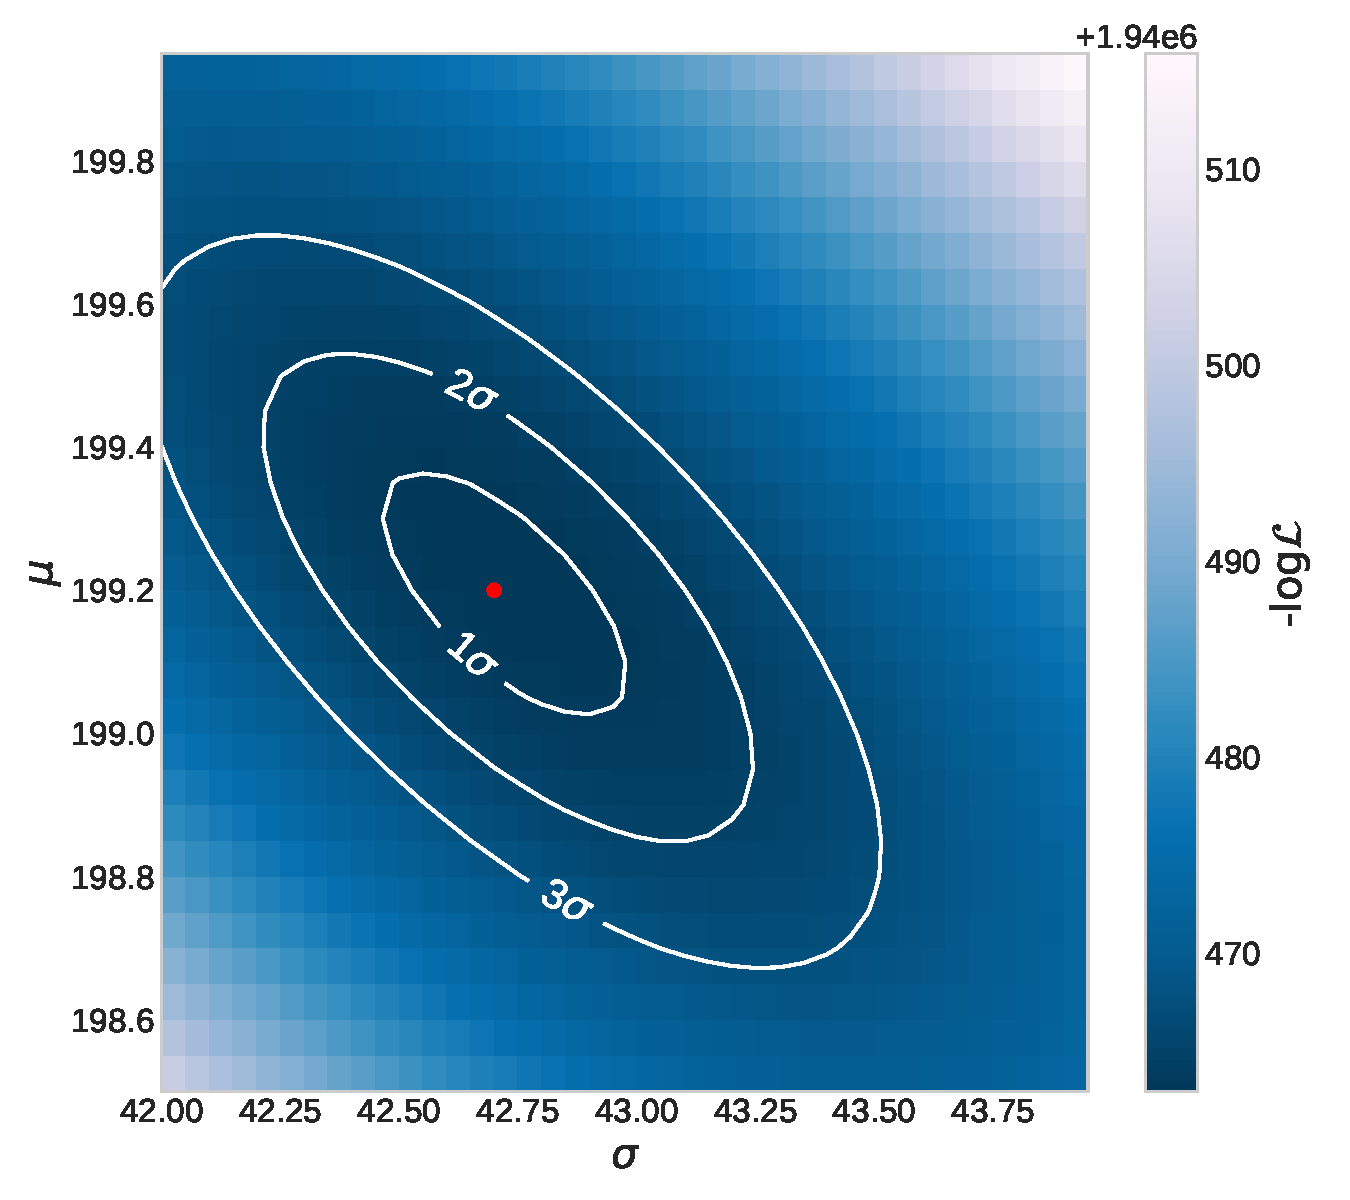
\includegraphics[width=0.45\textwidth]{exampleAnalysis/plots/Likelihood_Data_electron_VME.pdf}\hfill
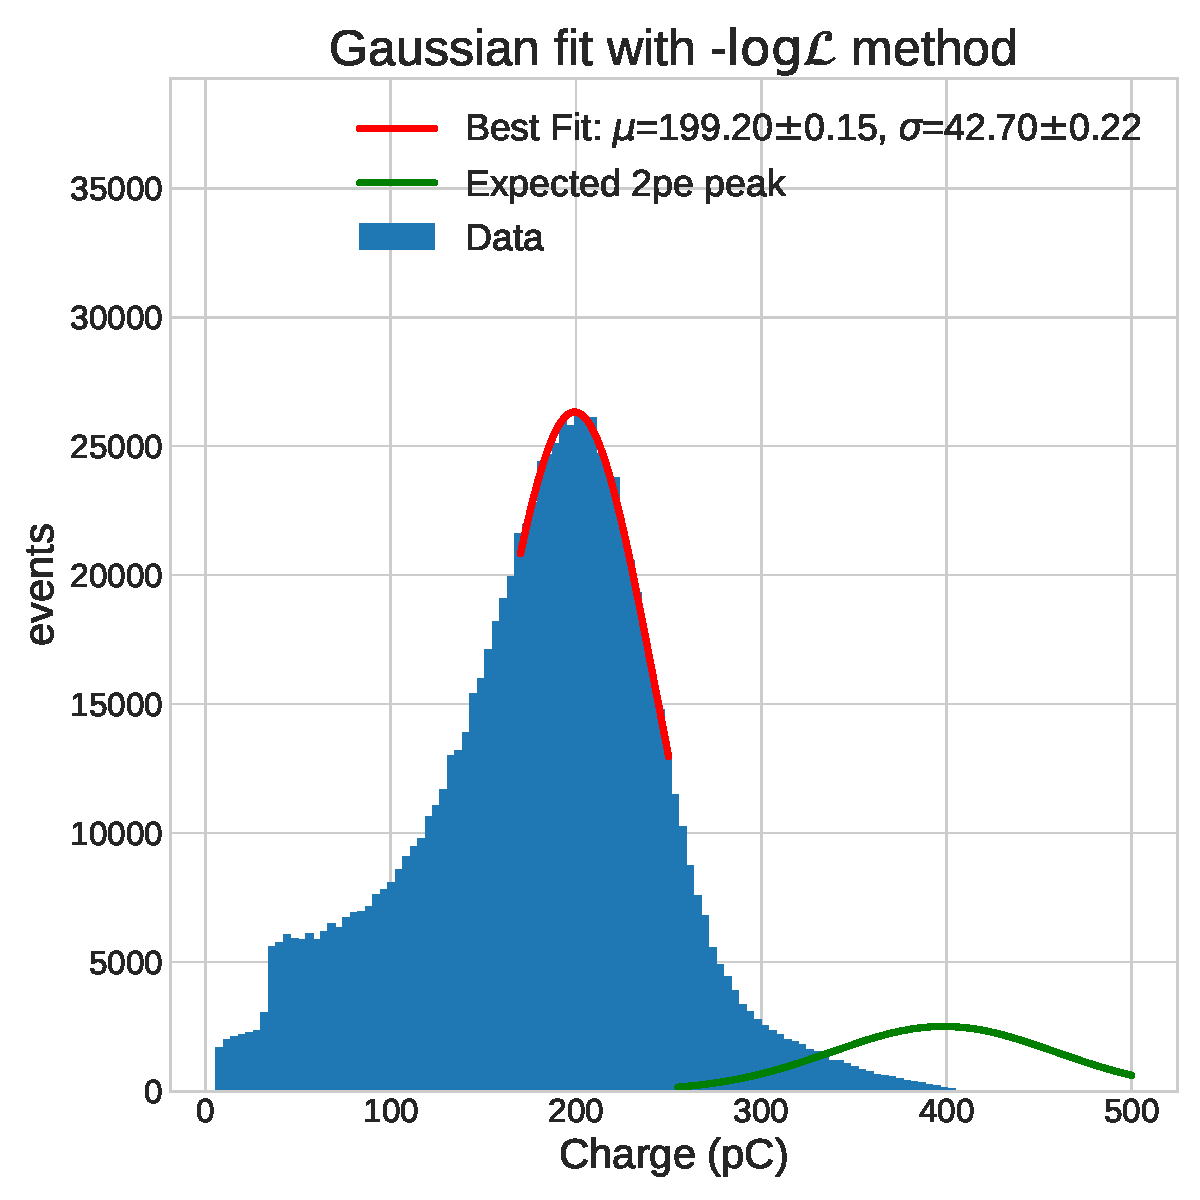
\includegraphics[width=0.45\textwidth]{exampleAnalysis/plots/LLH_Fit_electron_VME.pdf}
\begin{align*}
G &= \mu_{\text{best}}/e = 1242670 \\
\sigma_G &= \sigma_{\text{best}} / \mu_{\text{best}} = 21.44\%
\end{align*}
{\centering
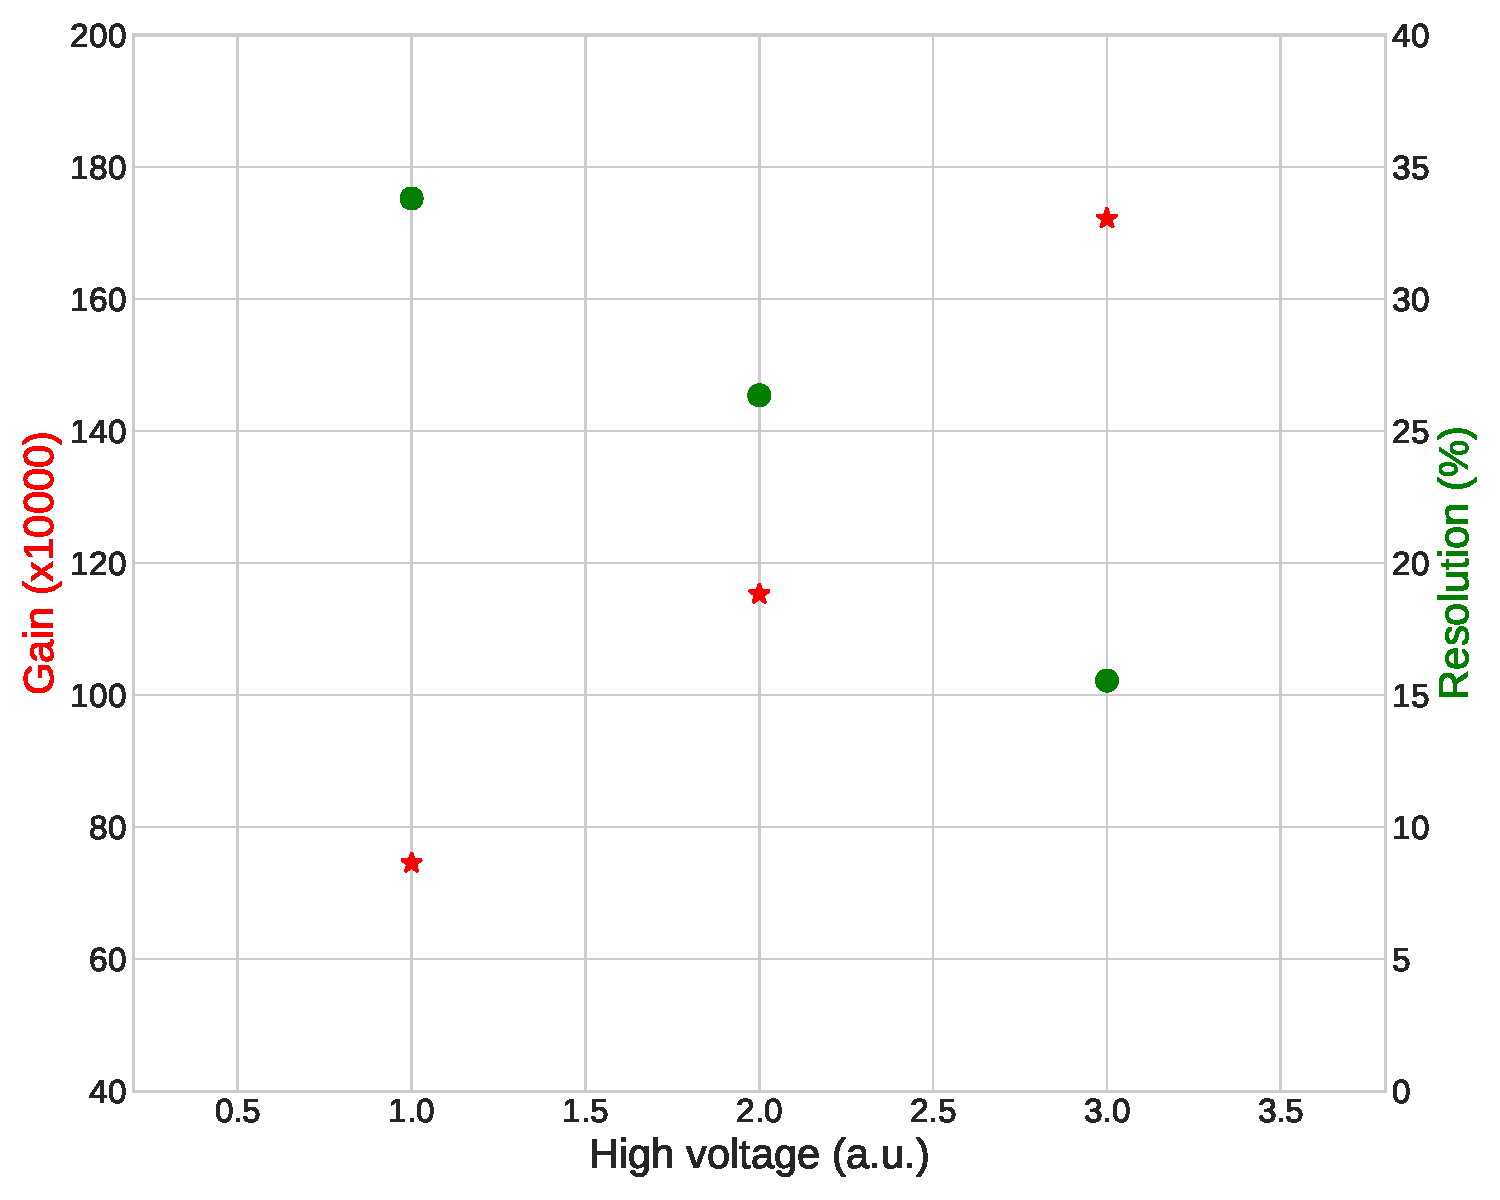
\includegraphics[width=0.7\textwidth]{exampleAnalysis/plots/Electron_Gain_Resolution_HV_VME.pdf}\\}
\end{additional}
}

